\documentclass[../CIT217_RHEL124_LabJournal.tex]{subfiles}

\begin{document}

%%%%%%%%%%%%%%%%%%%%%%%%%%%%%%%%%%%%%%%%%%%%%%%%%%%%%
%%%%%%%%%%%%%%%%%%%%%%%%%%%%%%%%%%%%%%%%%%%%%%%%%%%%%

\chapter[RHEL 124 Labs 7, 8, \& 9]{RHEL 124 \linebreak[1] Labs 7, 8, \& 9 \hspace*{\fill}{\date}}
\noindent\textbf{{RHEL 124 Labs} \hspace*{\fill}{\textbf{CIT 288}}}\linebreak[1]
{{Spring 2020} \hspace*{\fill}{Chaz Davis}}                             
%===================================
%===================================
\mysection{\textbf{Part 1: Chapter 7 Questions}}

\mysubsection{1}{Run the command sleep 1000 in the background. Using the ps
command, provide the output displaying it's still running.}
\\I ran {\scriptsize{\verb$sleep 1000$}\normalsize} into the terminal.
\\I then ran the command {\scriptsize{\verb$Ctrl + z$}\normalsize} to 
suspend the program and then {\scriptsize{\verb$bg$}\normalsize} to
put it into the background. 
\\Finally, I ran {\scriptsize{\verb$ps$}\normalsize} to show the running
processes on the system. The output you can see in
Fig.~\ref{Ch7}\subref{Ch7Sleep} on Pg.~\pageref{Ch7}.
\hfill\break

\noindent\mysubsection{2}{Abruptly terminate the sleep process that you created. Use the ps command to provide the output it is no longer running.}
\\First, I brought the sleep command back from the background to the foreground
using {\scriptsize{\verb$fg$}\normalsize}.
\\Then I used the key sequence {\scriptsize{\verb$Ctrl + C$}\normalsize} to
kill the foregrounded process.
\\Finally, I ran {\scriptsize{\verb$ps$}\normalsize} to show the running
processes on the system. The output you can see in
Fig.~\ref{Ch7}\subref{Ch7ps} on Pg.~\pageref{Ch7}.
\hfill\break

\noindent\mysubsection{3}{Provide the dynamic output of the top running processes on your system.}
\\First I opened a terminal and then ran the command {\scriptsize{\verb$top$}\normalsize}, 
the output of which you can see in Fig.~\ref{Ch7}\subref{Ch7Top} on Pg.~\pageref{Ch7}.

\begin{figure}[!b]\centering
\subfloat[Starting and verifying the Sleep 1000 process]{\label{Ch7Sleep}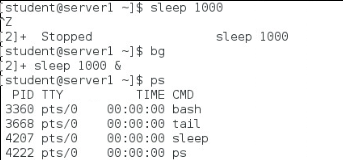
\includegraphics[width=.49\linewidth]{Figures/2020-02-13-114757_343x160_scrot.png}}\hfill
\subfloat[Terminating the sleep process]{\label{Ch7ps}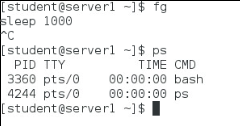
\includegraphics[width=.45\linewidth]{Figures/2020-02-13-114852_240x126_scrot.png}}\par 
\subfloat[Output of Top]{\label{Ch7Top}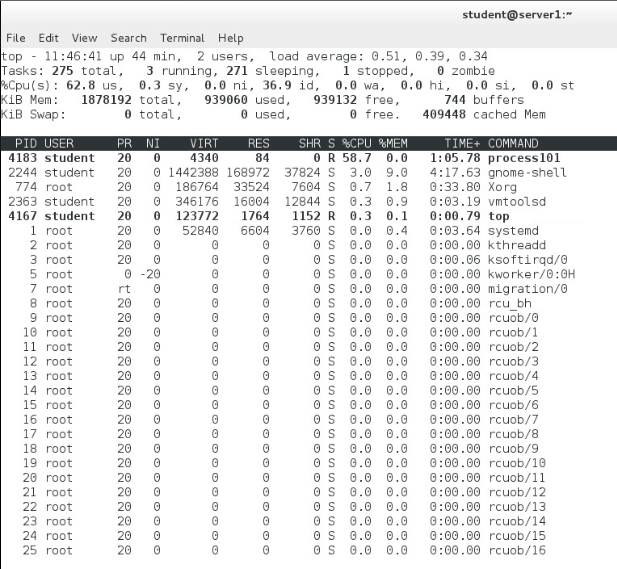
\includegraphics[width=.75\linewidth]{Figures/2020-02-13-114642_617x569_scrot.png}}\par
\caption{Chapter 7 Screenshots}
\label{Ch7}
\end{figure}
\clearpage

%===================================
\mysection{\textbf{Part 2: Chapter 8 Questions}}


\mysubsection{1}{Provide the output of the system status for the service firewalld.}
\\I went to the terminal on server1 and 
entered {\scriptsize{\verb$sudo systemctl status firewalld$}\normalsize}. 
\\I then entered my password.
\\Finally, I was given the output of the status of the firewall daemon see
Fig.~\ref{Ch8}\subref{Ch8.1}
\hfill\break

\noindent\mysubsection{2}{Is the service nfs enabled or disabled? Provide the output of its state.}
\\After logging into the terminal and entering the command
{\scriptsize{\verb$sudo systemctl status nfs$}\normalsize} and 
entering my credentials, we can now see in Fig.~\ref{Ch8}\subref{Ch8.2} that nfs is loaded but not active.
\\Alternatively, I could have run the command
{\scriptsize{\verb$sudo systemctl is-enabled nfs$}\normalsize} that output
is provided in Fig.~\ref{Ch8}\subref{Ch8.3}.


\begin{figure}[!hbt]\centering
\subfloat[Firewalld
status]{\label{Ch8.1}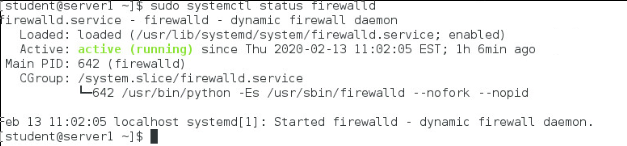
\includegraphics[width=.90\linewidth]{Figures/2020-02-13-120853_627x146_scrot.png}}\par
\subfloat[nfs Status]{\label{Ch8.2}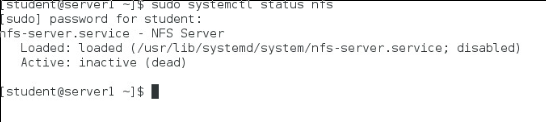
\includegraphics[width=.86\linewidth]{Figures/2020-02-13-123101_546x122_scrot.png}}\par
\subfloat[nfs is-enabled]{\label{Ch8.3}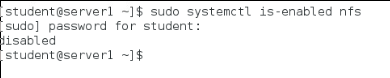
\includegraphics[width=.86\linewidth]{Figures/2020-02-13-123707_390x78_scrot.png}}\par
\caption{Chapter 8 Screenshots}
\label{Ch8}
\end{figure}

\clearpage

%===================================
\mysection{\textbf{Part 3: Chapter 9 Questions}}


\mysubsection{1}{ssh to server1 then run the hostname command. Provide the output.}
\\I logged into Desktop1 and opened a terminal. I then entered
{\scriptsize{\verb$ssh student@server1$}\normalsize} after confirmation and key
creation I was able to enter my password for the server account.
\\I then ran the command {\scriptsize{\verb$hostname$}\normalsize} the
output of which you can see in Fig.~\ref{Ch9}\subref{Ch9.1} on
Pg.~\pageref{Ch9}.
\hfill\break

\noindent\mysubsection{2}{Edit the sshd config file. Disable root logins. Disable strict modes. Provide the output of the file where this was accomplished.}
\\I logged into the server and used the command
{\scriptsize{\verb$sudo vim /etc/ssh/sshd_config$}\normalsize}
\\I then, went down to the authentication section, and changed the yes to a no
for both PermitRootLogin see Fig.~\ref{Ch9}\subref{Ch9.2} on
Pg.~\pageref{Ch9} and for StrictModes. See Fig.~\ref{Ch9}\subref{Ch9.3} on
Pg.~\pageref{Ch9}.
\hfill\break

\noindent Then to verify it took effect I used the command 
{\scriptsize{\verb$less /etc/ssh/sshd_config$}\normalsize} 
See Fig.~\ref{Ch9}\subref{Ch9.4} on
Pg.~\pageref{Ch9}.
\hfill\break

\noindent\mysubsection{3}{Generate an ssh key saved as your first name. Provide the output.}
\\I used the command {\scriptsize{\verb$ssh-keygen$}\normalsize} and
when prompted for file I told it to save as Chaz.
\\To verify this I used the command {\scriptsize{\verb$cat Chaz$}\normalsize},
the output is displayed in Fig.~\ref{Ch9}\subref{Ch9.5} on
Pg.~\pageref{Ch9}.

\begin{figure}[!hbt]\centering
\subfloat[Server1 hostname]{\label{Ch9.1}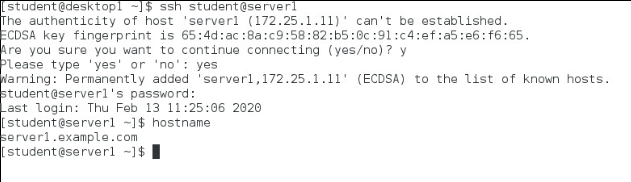
\includegraphics[width=.85\linewidth]{Figures/2020-02-13-124101_631x182_scrot.png}}\par
\subfloat[PermitRootLogin]{\label{Ch9.2}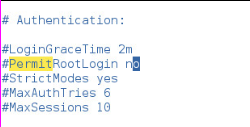
\includegraphics[width=.49\linewidth]{Figures/2020-02-13-132157_250x127_scrot.png}}\hfill
\subfloat[StrictModes]{\label{Ch9.3}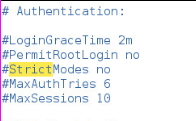
\includegraphics[width=.45\linewidth]{Figures/2020-02-13-132302_196x121_scrot.png}}\par
\subfloat[Less sshd config]{\label{Ch9.4}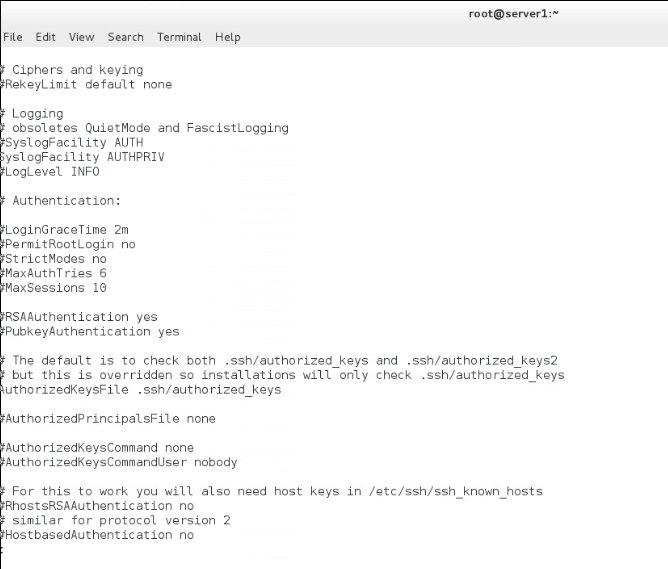
\includegraphics[width=.55\linewidth]{Figures/2020-02-13-132424_668x569_scrot.png}}\par
\subfloat[RSA ouput of Chaz]{\label{Ch9.5}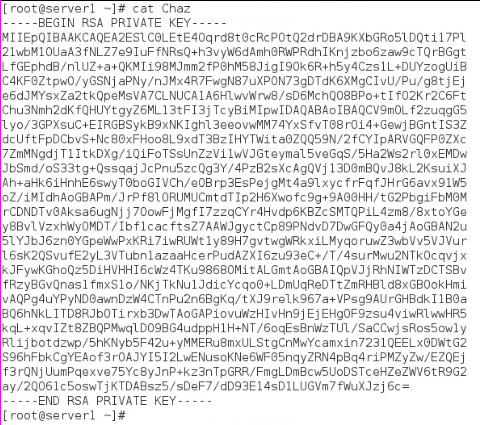
\includegraphics[width=.45\linewidth]{Figures/2020-02-13-132719_480x425_scrot.png}}\par
\caption{Chapter 9 screenshots}
\label{Ch9}
\end{figure}



%===================================

\end{document}
